\chapter{GPU Acceleration of FHI-aims}
\label{Sex:appendix_gpu_acceleration}

\section{Introduction}

\subsection{Overview of GPU Acceleration Philosophy in FHI-aims}

FHI-aims uses a batch integration scheme\cite{Havu08} in which the real-space integration points are broken up into spacially localized batches of points.  Each batch of points is assigned to an MPI rank, and each MPI rank processes its assigned batches sequentially.  After all batches have been processed, the MPI ranks communicate the final results to one another.

The batch integration scheme is at the heart of FHI-aims' O(N) scaling in number of atoms for most of the steps of the SCF cycle.  (An important exception is the solution of the Kohn-Sham equations, which will be addressed at the end of this section.)  Only basis elements that touch an integration point will contribute to the quantity being calculated for a given batch.  As basis elements have finite spacial extent, for a sufficiently large non-periodic system or unit cell of a periodic system, the number of basis elements needed for a given fixed-sized batch will be saturated.   Adding more atoms to the system, i.e. increasing the size of a non-periodic system or using a larger unit cell for a periodic system, will increase the number of batches linearly, but not the work done per batch, leading to linear scaling in number of atoms.  

By a happy accident, the batch integration scheme in FHI-aims lends itself naturally to GPU acceleration.  The details vary based on the task being accelerated, but the general strategy is:
\begin{enumerate}
	\item The MPI rank sets up a batch.
	\item The MPI rank communicates batch details to its assigned GPU.
	\item The GPU performs work on the batch.
	\item If the MPI rank needs to process the batch further, the GPU communicates the results back to its assigned MPI rank.
	\item After all batches have been processed, the GPU communicates its final results back to its assigned MPI rank.
\end{enumerate}

As each MPI rank processes its batch independent of other MPI ranks, no significant effort is needed to use GPU acceleration in an MPI environment.  The batches are small enough that they fit into memory on a NVidia Kepler Tesla GPU.  As each batch is statistically similar in size, the memory usage of a given batch is independent of system size; the GPU will not run out of memory as the system size increases for a fixed number of MPI ranks.  Furthermore, most of the computation time for tasks utilizing the batch integration scheme is taken up by a small number of BLAS/LAPACK subroutine calls occurring at the end of the batch processing.  These subroutine calls can be easily replaced by cuBLAS (\url{https://developer.nvidia.com/cublas}) calls.

The pseudocode for this process is:
\begin{verbatim}
  do i_batch = 1, n_batches
    set_up_batch_on_cpu
    copy_batch_information_to_gpu
    call cuBLAS_Function()
    if gpu_data_needed_on_cpu
      copy_partial_gpu_data_back_to_cpu  
      cpu_performs_work_on_partial_gpu_data
    end if
  end do

  copy_gpu_final_data_back_to_cpu
\end{verbatim}

\subsection{Current State of GPU Acceleration in FHI-aims}

The steps needs to use GPU acceleration in FHI-aims are:
\begin{enumerate}
	\item Make sure prerequisites are installed.
	\item Modify \texttt{make.sys} to include GPU acceleration flags.
	\item Compile FHI-aims as normal, optionally linking against GPU-accelerated ELPA via ELSI (see next subsection).
	\item Add GPU acceleration keywords to \texttt{control.in}.
	\item Run FHI-aims as normal.
\end{enumerate}
It cannot be stressed enough that the user should consult the documentation for their architecture, as their architecture may require additional steps to use GPU acceleration beyond what is listed here.

The GPU acceleration code is considered stable and suitable for production calculations.  An example scaling plot for timings of the first SCF step for 128 atoms of GaAs on Titan Cray XK7 is shown in Figure \ref{fig:GPU_Scaling}.  We generally find that the charge density update shows the largest GPU acceleration speed-up.  

Larger speed-ups are observed as the basis set size is increased.  If a non-periodic system or unit cell of a periodic system is too small (say, a primitive cell of GaAs running on 32 MPI ranks), a slow-down may actually be observed.

\begin{figure}
  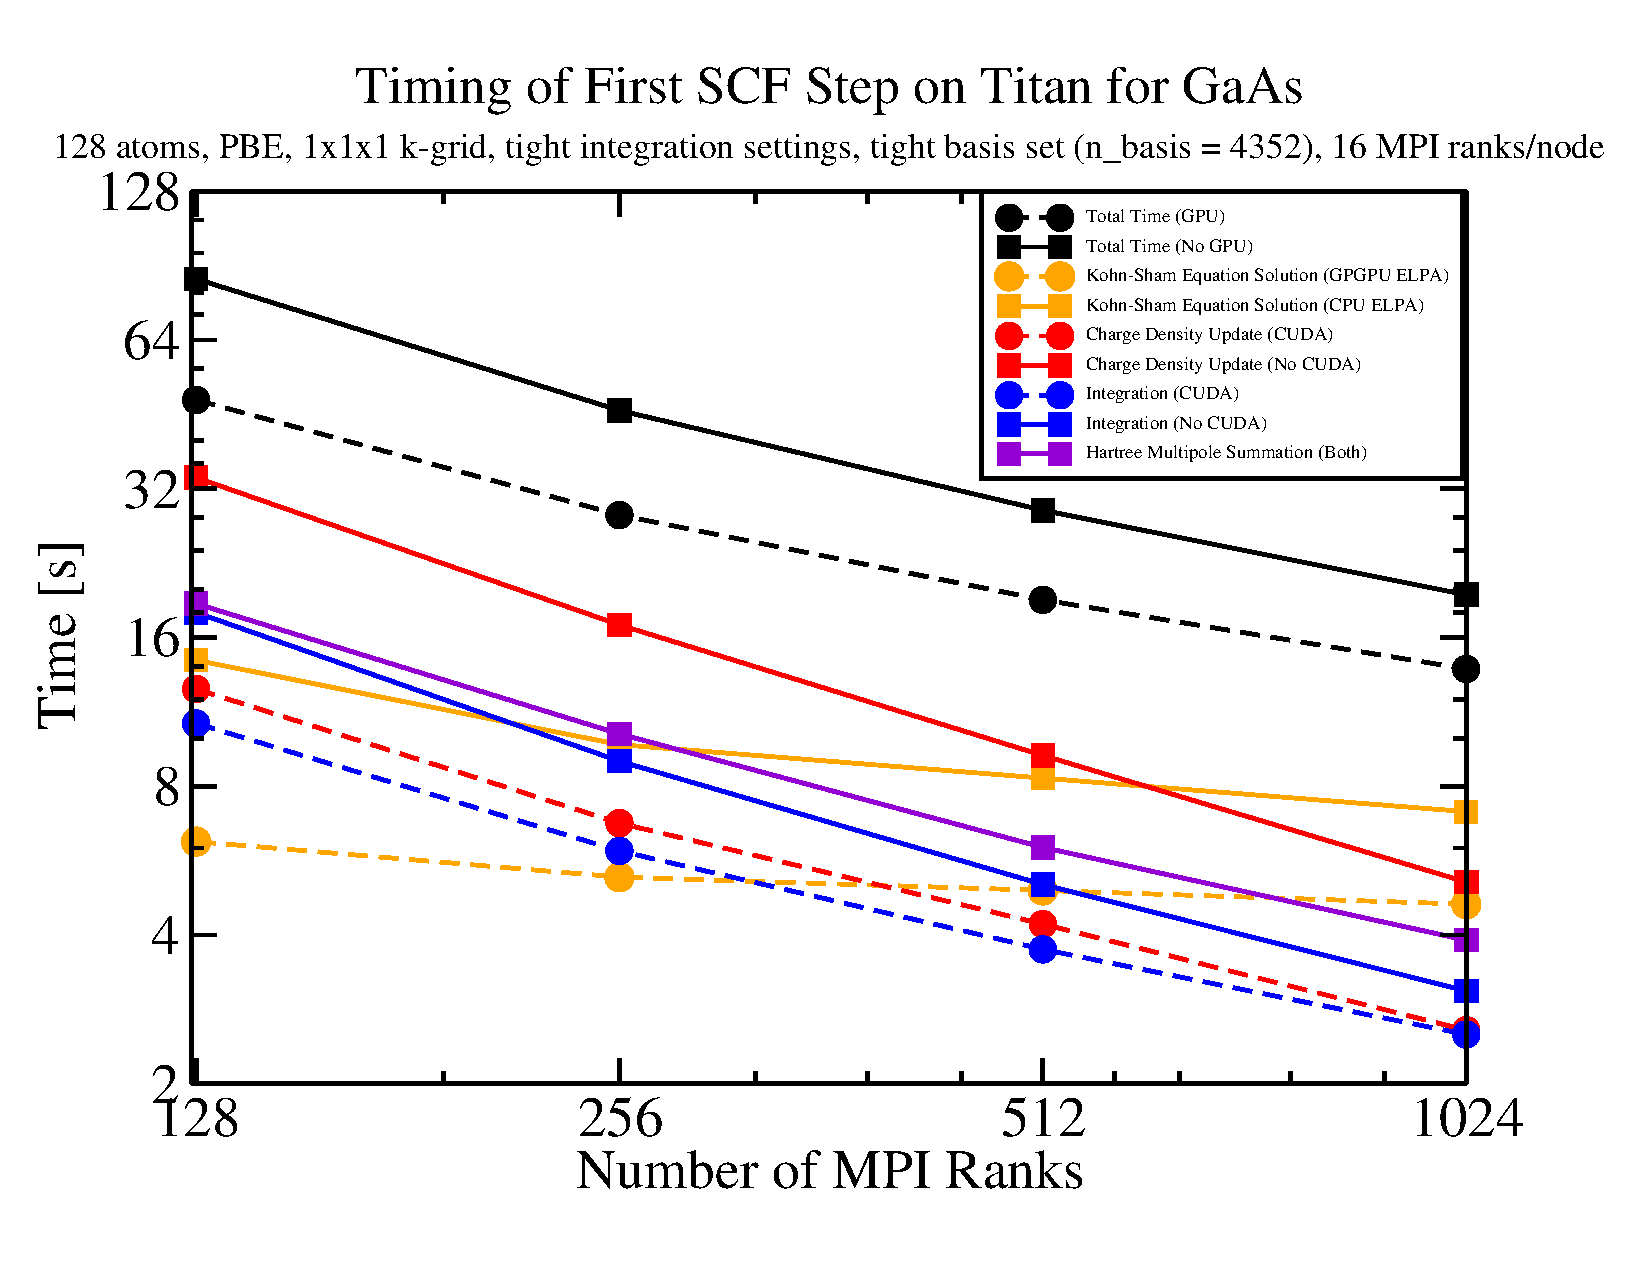
\includegraphics[width=\linewidth]{GaAs_4x4x4Supercell_NoPrecond_GPUBatchSize200}
  \caption{Example scaling plot for GPU acceleration.  The solid lines are CPU-only calculations, and the dotted lines are GPU-accelerated calculations.  At present, there is no GPU acceleration in the Hartree multipole summation, so both CPU-only and GPU-accelerated calculations have the same timings for this task.}
    \label{fig:GPU_Scaling}
\end{figure}

The list of tasks we have GPU accelerated natively in FHI-aims is:
\begin{itemize}
	\item Integration of the Hamiltonian matrix
	\item Charge density update via density matrices
	\item Pulay forces (not tested!)
\end{itemize}
In the future, we plan to natively GPU accelerate the following tasks:
\begin{itemize}
	\item Hartree multipole summation
	\item Construction of the Fock matrix (for HF/hybrid-functional calculations and beyond)
\end{itemize}

\subsection{GPU Acceleration of the Solution of the Kohn-Sham Equation: ELSI}
For small and mid-sized DFT-GGA calculations with no relaxation, the charge density update and Hamiltonian integration collectively dominate the computational time of a calculation.  For larger systems, the solution of the Kohn-Sham equation dominates computational time due to the O(N$^3$) scaling of ELPA, the eigensolver implemented in FHI-aims.  The rate-limiting nature of the solution of the Kohn-Sham equation is an impediment common to all Kohn-Sham DFT codes.  The ubiquity of this problem has spurred the creation of the ELectronic Structure Infrastructure (ELSI), a collection of methods that solve or circumvent the eigenvalue problem combined with a flexible interface layer to allow for usage by multiple Kohn-Sham DFT codes.   More information may be found at the ELSI Interchange (\url{http://elsi-interchange.org}).

One major goal of ELSI is support for next-generation technologies, including GPU acceleration.  FHI-aims does not natively accelerate the solution of the Kohn-Sham equation, but rather it uses ELSI for this task.  In the future, ELSI will be distributed with FHI-aims; as of this writing, using ELSI requires that the user manually install and link FHI-aims against it.  The steps are:
\begin{enumerate}
	\item Download ELSI from its GitLab repo (\url{http://www.elsi-interchange.org:81/users/sign_in})
	\item Select the GPU kernel for ELPA by setting \texttt{ARCHITECTURE = GPU} in ELSI's \texttt{make.sys} file
	\item Install ELSI
	\item Link FHI-aims against ELSI 
	\item Run GPU-accelerated ELPA via ELSI by setting flags in \texttt{control.in}
\end{enumerate}
We stress that these steps are only necessary for GPU acceleration of the solution of the Kohn-Sham equations.  For more information, please see the ELSI Interchange.

\section{Prerequisites}
We have tested the GPU acceleration code on NVidia K20X, K40m, K40c, and P100 GPUs.  There are no plans to support ATI Radeon GPUs.

To compile FHI-aims with GPU acceleration, three additional packages are needed beyond the usual packages for a standard FHI-aims install.  These packages are:
\begin{itemize}
	\item A C compiler
	\item The CUDA Toolkit, supplied by NVidia at \url{https://developer.nvidia.com/cuda-toolkit}
	\item NVidia Multi-Process Service (MPS), installed as part of the CUDA Toolkit
\end{itemize}
These packages should be available on any properly configured GPU-accelerated architecture.

The bulk of the testing of the GPU acceleration code was performed with CUDA 7.5, but code development and early testing used CUDA versions ranging from 5.5 to 7.0.  We anticipate that the GPU acceleration in FHI-aims should continue to work with these CUDA versions.

\section{Installation}
Compiling the FHI-aims executable with support for GPU acceleration requires a set of GPU acceleration flags be included in the \texttt{make.sys} file.  The installation procedure is otherwise the same as a standard FHI-aims installation.  We have only tested the GPU code for the scalapack.mpi target, but it should work for any target.

\subsection{GPU Acceleration Flags in \texttt{make.sys}}

The flags needed in \texttt{make.sys} are:
\begin{itemize}
	\item USE\_C\_FILES: Instructs the make process that C files should be compiled.  This must be set to ``yes''. 
	\item CC: The C compiler
	\item CCFLAGS: Optimization flags for compiling C code.
	\item CUDAROOT: The root directory of the CUDA Toolkit.
	\item CUDACC: The location of nvcc, the CUDA compiler driver.  For a standard installation of the CUDA Toolkit, the value of this flag will be \$CUDAROOT/bin/nvcc.
	\item USE\_CUDA: Instructs the make process that CUDA files should be compiled.  This must be set to ``yes''.
	\item CUDAFLAGS:   Optimization flags for compiling CUDA code.  \textbf{This will be architecture-dependent!}
	\item CUDALIBS:    The locations of required CUDA libraries.  The GPU acceleration in FHI-aims uses the CUDA Runtime and cuBLAS libraries.  For a standard installation of the CUDA Toolkit, they will be located in \$CUDAROOT/lib64 and have the filenames libcudart.so and libcublas.so, respectively.
\end{itemize}

\subsection{Example \texttt{make.sys} Fragments for GPU Acceleration}

Below are two \texttt{make.sys} fragments for different architectures provided for use as templates.  The first fragment is for Timewarp, the private cluster of the FHI-aims group at Duke University, and the second is for Oak Ridge National Laboratory's Titan Cray XK7.  Titan uses wrappers for compilation, hence the absence of various flags seen in the Timewarp \texttt{make.sys} fragment.  The Timewarp \texttt{make.sys} fragment is the more ``complete'' of the two and should be used as the main template.  \textbf{These fragments should be used as templates for the user's \texttt{make.sys}; if these fragments are simply copy-and-paste'd into the user's \texttt{make.sys}, the code will almost certainly fail to compile.}  We encourage users to put their own GPU acceleration compilation flags on the ``Known compiler settings'' section of the aimsclub wiki (\url{https://aimsclub.fhi-berlin.mpg.de/wiki/index.php/Known\_compiler\_options}).

\subsubsection{Timewarp}

Architecture of a Node:
\begin{itemize}
	\item CentOS release 6.5
	\item Dual Intel Xeon E5-2670v2
	\item 2 x NVidia Tesla K40 (K40m and K40c)
	\item Intel Fortran 14.0.1
\end{itemize}

\begin{verbatim}
Relevant portion of make.sys:

###############
# C,C++ Flags #
###############
 USE_C_FILES = yes 
 CC          = gcc 
 CXX         = g++ 
 CCFLAGS     = -O3 -mavx 
 CXXFLAGS    = -O3 -mavx

##############
# CUDA Flags #
##############
 CUDAROOT  = /usr/local/cuda-7.5
 CUDACC    = ${CUDAROOT}/bin/nvcc
 USE_CUDA  = yes
 CUDAFLAGS = -O3 -c -m64 -arch=sm_35
 CUDALIBS  = -lstdc++ \
             --ptxas-options=-v --use_fast_math \
             -L${CUDAROOT}/lib64 \
             -Xlinker -rpath ${CUDAROOT}/lib64 \
             -lcudart -lcublas
\end{verbatim}

\subsubsection{Titan Cray XK7}

Architecture of a Node:
\begin{itemize}
	\item Cray XK7 Architecture
	\item AMD Opteron 6274 16-core CPU
	\item NVidia Tesla K20X GPU
	\item PGI 16.7 compiler
\end{itemize}

\begin{verbatim}
Relevant portion of make.sys:

###############
# C,C++ Flags #
###############
 USE_C_FILES = yes
 CC = cc
 CCFLAGS = -O0
 CXX = CC
 CXXFLAGS = -O0

##############    
# CUDA Flags #
##############
# CUDA Files
 CUDAROOT = /opt/nvidia/cudatoolkit7.5/7.5.18-1.0502.10743.2.1
 CUDACC = ${CUDAROOT}/bin/nvcc
 USE_CUDA = yes 
 CUDAFLAGS = -O3 -c -m64 -arch=sm_35
 CUDALIBS = -lcublas
\end{verbatim}

\section{Running FHI-aims with GPU Acceleration}
Compiling the FHI-aims executable with GPU acceleration support will not automatically turn on GPU acceleration.  To use GPU acceleration when running FHI-aims, the user specifies which tasks should be GPU accelerated independently using keywords specified in \texttt{control.in}.  The keywords controlling GPU acceleration are:

\keydefinition{gpu\_density}{control.in}
{
  \noindent
  Usage: \keyword{gpu\_density} \\[1.0ex]
  Purpose: Use GPU acceleration when updating the charge density via density matrices.  This keyword does nothing when using orbital-based density update.  \\[1.0ex] 
}


\keydefinition{gpu\_hamiltonian}{control.in}
{
  \noindent
  Usage: \keyword{gpu\_hamiltonian} \\[1.0ex]
  Purpose: Use GPU acceleration when integrating the Hamiltonian matrix.  \\[1.0ex] 
}

\keydefinition{gpu\_pulay}{control.in}
{
  \noindent
  Usage: \keyword{gpu\_pulay} \\[1.0ex]
  Purpose: Use GPU acceleration when calculating Pulay forces.  This keyword has not been tested, and it is not recommended that it be used.  \\[1.0ex] 
}

An example fragment for \texttt{control.in} to enable GPU acceleration of the charge density update and Hamiltonian integration is:
\begin{verbatim}
********************
* GPU Acceleration *
********************
gpu_density
gpu_hamiltonian
\end{verbatim}
	
One important keyword when running GPU-accelerated calculations is \keyword{points\_in\_batch}, which sets the targeted number of points per batch.  This parameter is a trade-off: increasing the number of points per batch increases the work done by the GPU per batch, increasing the efficiency of the GPU, but it also increases the number of basis elements interacting with a batch, increasing the memory usage.  Due to technical details, some of this additional work is unnecessary, as it does not appreciably add to the integrals being evaluated.

The default value for \keyword{points\_in\_batch} based on early CPU-only benchmarks was set to 100.  We have found that increasing this value to 200 is a better choice for our test architecture (Kepler Tesla GPUs) when using GPU acceleration, and we have set 200 as the default value when running any GPU-accelerating any tasks involving the batch integration scheme.  The user should also play around with this parameter for their own architecture, particularly if they are using a different GPU architecture.

All GPU keywords may be set independently.  We have found that the charge density update shows a significantly higher GPU-accelerated speed-up than the Hamiltonian integration (c.f. Figure \ref{fig:GPU_Scaling}).  If the user's architecture uses fast CPUs but slow GPUs, enabling GPU acceleration for the Hamiltonian integration may actually slow down the calculation.

\subsection{Memory Usage with GPU Acceleration}

One hypothetical limitation in the current implementation of GPU acceleration in FHI-aims is GPU memory usage.  All MPI ranks are assigned to one of the available GPUs, implying that a GPU will generally have more than one MPI rank assigned to it.  All MPI ranks will offload their work during the compute-intensive cuBLAS call onto the assigned GPU.  This creates two bottlenecks:  not only do MPI ranks need to ``wait their turn'' behind other MPI ranks before the GPU processes their current batch, but each MPI rank will take up a portion of the GPU's memory.  If a calculation runs out of memory when using GPU acceleration, some possible solutions are:
\begin{itemize}
	\item Reduce the basis set density, if possible.  This should only be done if additional basis set elements were uncommented in the species defaults; we do not recommend the user uses less basis elements than the default ``tight'' basis set unless they know exactly what they're doing.
	\item Read Section \ref{Sec:Large-scale}, ``Large-scale, massively parallel: Memory use, sparsity, communication, etc.'' of the manual.  In particular, consider setting \keyword{use\_local\_index} to \texttt{.true.} .  While there will be a time cost associated with enabling this keyword,  the memory savings can be considerable.
	\item Use less MPI ranks per node.  By having less MPI ranks per node, less MPI ranks will be bound to the GPUs on each node, reducing the overall GPU memory usage.
\end{itemize}
In the future, we will be addressing the memory issue by refining our load balancing infrastructure to assign only one MPI rank to each GPU, but giving more batches to the MPI rank to compensate.

\subsection*{Summary}
\begin{itemize}
	\item Use keywords in \texttt{control.in} to enable GPU acceleration.
	\item Optimize \keyword{points\_in\_batch} for the architecture used.
	\item Test each GPU acceleration keyword individually to make sure there is a speed up compared to the CPU-only version for the architecture used. 
	\item Reduce the basis set size or set \keyword{use\_local\_index} to \texttt{.true.} if your calculation runs out of memory.  (This is true for all calculations, not just GPU-accelerated calculations.)
\end{itemize}
